\documentclass[a4paper,12pt]{article}
\usepackage{graphicx}
\usepackage[utf8]{inputenc}
\usepackage[T1]{fontenc}
\usepackage{geometry}
\usepackage{multicol}
\usepackage{amsmath,tkz-tab}
\geometry{top=2cm, bottom=2cm, left=2cm, right=2cm}

\begin{document}

\noindent
\begin{minipage}[t]{0.48\textwidth}
\raggedright
\textbf{Ministère de l'Éducation Nationale}\\
Inspection Académique de Kédougou\\
Lycée Dindéfelo\\
Cellule de Mathématiques
\end{minipage}
\hfill
\begin{minipage}[t]{0.48\textwidth}
\raggedleft
\textbf{Année scolaire 2024-2025}\\
Date : 17/10/2024\\
Classe : Terminale S2\\
Professeur : M. BA
\end{minipage}

\vspace{1cm}
\section*{Exercice 1}

1. Déterminer, si elles existent, les limites suivantes :

\[
\lim_{x \to 0} \frac{\tan(3x)}{1 - \sqrt{x + 1}} \quad ; \quad \lim_{x \to 2} \frac{\sqrt{x+2} - \sqrt{3x+3}}{x-2} \quad ; \quad \lim_{x \to 0} \frac{\cos x - 1}{x^3 + x^2}
\]

\[
\lim_{x \to 0} \frac{3 \sin^2 x - \cos x + 1}{x^2} \quad ; \quad \lim_{x \to 0} \frac{\sin x - \tan x}{x^3}\quad ; \quad\lim_{x \to 0} \frac{1 - \cos x}{x \tan x}
\]

2. Déterminer, si elles existent, les limites suivantes :

\[
\lim_{x \to \frac{\pi}{2}} \frac{1 - \tan x}{1 + \tan x}\quad ; \quad \lim_{x \to 3} \frac{\sqrt{x+1} - 2}{\sqrt{x^2 - x - 6}}\quad ; \quad\lim_{x \to 1} \frac{\sqrt{x+3} - \sqrt{5-x}}{\sqrt{2x+7} - \sqrt{10-x}}
\]
\[
\lim_{x \to 0} \frac{\sqrt{1+\sin x -1}}{\sin 2x}\quad ; \quad\lim_{x \to \frac{\pi}{2}} \frac{\cos x}{1-\sin x}
\]

3. Déterminer, si elles existent, les limites suivantes :

\[
\lim_{x \to \pm \infty} \left(x - \sqrt{x^2 + 3x - 1}\right)\quad; \quad \lim_{x \to \pm \infty} \frac{2x + \sqrt{x^2 + 1}}{x}\quad; \quad
\lim_{x \to \pm \infty} \frac{x+1}{\sqrt{x+3}-2}
\]

\[
\lim_{x \to \pm \infty} \left(2x + \sqrt{x - 1}\right)\quad; \quad
\lim_{x \to \pm \infty} \left(x + \sqrt{2x^{2} - 5x + 1 }\right)\quad; \quad
\lim_{x \to \pm \infty} \left(x\sqrt{\frac{x+1}{x-1}}\right)
\]

\[
\lim_{x \to \pm \infty} \frac{x - \sqrt{|x|}}{3x + 2}
\]

4. Déterminer, si elles existent, les limites suivantes :
\[
\lim_{x \to \pm \infty} \frac{x^2 + \sin x}{x} \quad ; \quad \lim_{x \to \pm\infty} \frac{x + \sin x}{2 - \sin x} \quad ; \quad \lim_{x \to \pm \infty} \frac{x^3}{3 + 2 \sin x}
\]

5. Déterminer les réels \( a \) et \( b \) pour que la droite d'équation \( y = ax + b \) soit une asymptote à la courbe représentative de la fonction \( x \mapsto \sqrt{x^2 + 4} - \frac{x}{\sqrt{2}} \).

\section*{Exercice 2}

Calculer les limites suivantes :

\[
1. \quad \lim_{x \to \frac{\pi}{4}} \frac{2 \cos x - \sqrt{2}}{x - \frac{\pi}{4}} \quad ; \quad \lim_{x \to 1} \frac{\sin(\pi x)}{x - 1}
\]

\[
2. \quad \lim_{x \to \frac{\pi}{4}} \frac{1 - \sqrt{2} \cos x}{1 - \sqrt{2} \sin x} \quad ; \quad \lim_{x \to 0^+} \frac{x \cos x + \sin x}{\sqrt{x + 1} - 1} \\
\]
\[
3. \quad \lim_{x \to \frac{\pi}{4}} \frac{\tan x - 1}{x - \frac{\pi}{4}} \quad ; \quad \lim_{x \to 0} \frac{1}{x^2} \left( \frac{2}{\cos x }+ \cos x - 3 \right)
\]
\[
4. \quad \lim_{x \to +\infty} \left( x \arctan (\sqrt{x}) - \frac{\pi}{2} x \right) \quad ; \quad \lim_{x \to 0^+} \frac{1}{x} \arctan \left( \frac{\sqrt{x}}{x + 1} \right)
\]

\[
5. \quad \lim_{|x| \to +\infty} \left( 3x - 1 + \sqrt{9x^2 + 3x - 2} \right) \quad ; \quad \lim_{x \to 0} \frac{1 - x^2 E \left( \frac{1}{x} \right)}{1 + x^2 E \left( \frac{1}{x} \right)} 
\]

\section*{Exercice 3}

Étudier la continuité de la fonction $f$ sur $D_f$ dans chaque cas.

1. $f(x) = x + \sqrt{x+1}$.

2. $f(x) = 4x + 1 + \frac{1}{x - 1}$.

3. $f(x) = 2\sqrt{x} - x$.

4. $f(x) = \frac{\sqrt{1 + x}}{1 - x}$.

\section*{Exercice 4}


Donner la dérivée des fonctions définies par :

\[
f(x) = \frac{1 + \cos(2x)}{1 - \sin(2x)} \quad ; \quad
g(x) = \left( x + \frac{1}{x} \right) \sqrt{\frac{1}{x}} \quad ; \quad
h(x) = \sqrt[3]{x - 6} + \frac{1}{x} \quad ; \quad
k(x) = \left| \frac{x^2 - x}{x - 1} \right|
\]

\[
m(x) = x \sqrt{\frac{x^2 - 1}{x^2 + 1}} \quad ; \quad
n(x) = \frac{\sqrt{x^2 - 3x + 2}}{x + 1} \quad ; \quad
p(x) = \frac{\tan x}{1 - 2 \sin x}
\]

\[
q(x) = 3 \left( x^2 - 3x + 5 \right)^4 \quad ; \quad
r(x) = \cos^2(3x) \quad ; \quad
s(x) = -2 \tan^2(2x)
\]
\newpage
\section*{Exercice 5}
Etude d'une fonction par lecture graphique
\begin{figure}[h]
\centering
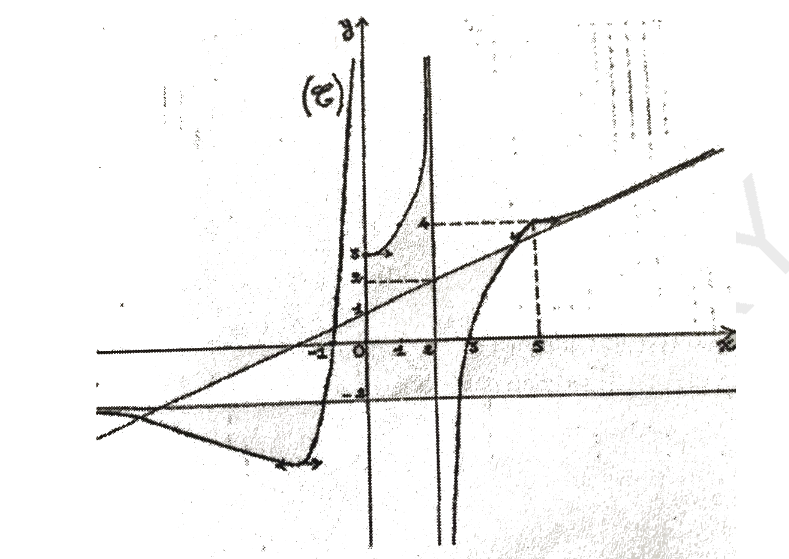
\includegraphics[width=0.8\textwidth]{courbe.png}
\caption{Courbe de (Cf)}
\label{fig:monimage}
\end{figure}
%\includegraphics[scale=0.8]{c1c2c3.png}
La courbe $(C_f)$ ci-dessus est celle d'une fonction $f$ dans un repère orthonormé. $f$ est définie en 0 et on a : $f(0) = 3$.

\begin{enumerate}
    \item Préciser l'ensemble de définition de $f$.
    \item Donner les limites suivantes :
    \[
    \textbf{a)} \lim_{x \to +\infty} f(x), \quad \lim_{x \to -\infty} f(x) ;
    \]
    \[
    \textbf{b)} \lim_{x \to 0^+} f(x), \quad \lim_{x \to 0^-} f(x) ;
    \]
    \[
    \textbf{c)} \lim_{x \to 2^+} f(x), \quad \lim_{x \to 2^-} f(x) ;
    \]
    \item La courbe admet-elle une asymptote oblique ? Si oui, donner son équation.
    \item Préciser les équations des autres asymptotes.
    \item La fonction $f$ est-elle dérivable en 5 ? Justifier la réponse.
    \item Dresser le tableau de variation de $f$.
\end{enumerate}


\end{document}
